\documentclass[a4paper]{article}

\setcounter{secnumdepth}{0}

%Metadata
\title{Kuwaiba Open Inventory Deployment Manual}
\author{Neotropic SAS}
\date{27.07.2016}

%Imports
\usepackage{graphicx}
\usepackage[utf8]{inputenc}
\usepackage{booktabs}
\usepackage[margin=3cm]{geometry}
\usepackage{color}
\usepackage{framed}
\usepackage{verbatimbox}
\usepackage[toc,page]{appendix}
\usepackage{nameref}
\usepackage{textcomp}
\usepackage{pdflscape}
%\usepackage{hyperref}

%Modify some defaults
\setlength{\parindent}{0pt} %don't indent new paragraphs

\begin{document}
	\maketitle
	\pagenumbering{gobble}
	
	\begin{figure}[b]
		\centering System Version \textbf{1.0}
			
		Visit \textbf{kuwaiba.org} for documentation, latest updates and upcoming events
	\end{figure}

	\newpage
	
	\tableofcontents

	\newpage
	\section{Document History}
		\begin{table}[h!]
			\centering
			\begin{tabular}{l||p{10cm}} %Each letter tells the parser what alignment should have every column
				\toprule
				\textbf{Date} & \textbf{Comments}  \\
				\midrule
				August 3rd 2016 & First version adapted to Kuwaiba 1.0, this documentation was created with LaTeX\\
				\bottomrule
			\end{tabular}	
				
		\end{table}
	\newpage
	\section{License}
		\begin{table}[ht]
			\centering
			\begin{tabular}{cp{10cm}}
				
				
\includegraphics[]{img/cc_license_logo.jpg} & This document is published under the terms of a license Creative Commons by-nc-sa. You can find details about it at\linebreak
				\textbf{http://creativecommons.org/licenses/by-nc-sa/2.0/ } \\

				
\includegraphics[width=2cm]{img/osi_logo.jpg} & Kuwaiba Server and Client are licensed under EPL v1 and GPL v2. You can find the whole text of this licenses at \linebreak
				\textbf{http://www.eclipse.org/legal/epl-v10.html} \linebreak
				\textbf{http://www.gnu.org/licenses/old-licenses/gpl-2.0.html} \\
			\end{tabular}
		\end{table}
		\paragraph{Disclaimer} \hspace{0pt}
		\begin{itemize}
			
		
			\item This document is provided “as is”, with no warranty at all. Install the software and follow the instructions included at your own risk.
			
			\item Kuwaiba uses third-party components with compatible open source licenses (LGPL, BSD-like, etc). You can find a complete list at the project's web page.
		\end{itemize}
	
	\newpage
	\pagenumbering{arabic}
   	
   	To deploy kuwaiba into a server you must have in consideration.

	\section{Dependecies} \label{sec:dependencies}
		The installers of the dependencies need it by kuwaiba to work properly such as a JDK, an Application Server(Glassfish), a database engine(Neo4j), were located in compressed files in the path: \textit{/data/installs/dependencies/} in this directory you will find:
		\begin{itemize}
			\item The \textbf{JDK}, the jdk-7u65\_x64, this is the selected and tested JDK for kuwaiba v1.0.
			\item The \textbf{Java Server Application}, Glassfish 4.1.1
			\item The \textbf{Database}, Neo4j 2.3.3.
		\end{itemize}
	
	\section{Directory Structure for Kuwaiba} \label{sec:directories_structure}
		The directory structure used to deploy kuwaiba were: 
		\begin{itemize}
			\item In \textbf{/opt/glassfish4}, were located the the Java Server Application used to deploy the kuwaiba instance, GlassFish 4.1.1 (The server was setup as a service, you can only start/restar/stop it as a root, see \textbf{\nameref{sec:glassfish_as_service}}). 
			\item In \textbf{/opt/jdk7u65}, were located the JDK that uses kuwaiba.
			\item In \textbf{/data/installs/kuwaiba/} You will find two directories \textbf{dev/} and \textbf{0.7.1/} both contains different versions of the kuwaiba's installer, actually is deployed one ithe file with the last date in the \textbf{dev/} directory.
			\item In \textbf{/data/db/kuwaiba.db} were located all the data produce by Kuwaiba.
			\item In \textbf{/data/img/backgrounds} are stored all the images that kuwaiba's users load in the modules that let the usage of backgrounds 
			\item In \textbf{/data/backups/db} will be stored a backup of Kuwaiba's database. (This backups will be done periodically by a script see \textbf{\nameref{sec:backup_script}}). 
			\item In \textbf{/data/backups/backgrounds} will be stored the backgrounds used some modules of kuwaiba (This backups will be done periodically by a script see \textbf{\nameref{sec:backup_script}}). 
	    \end{itemize}

	\section{Third party Libraries in Kuwaiba} \label{sec:third_party_libs}
		\subsection{Database}
	    In the final kuwaiba's installer we don't include the libraries of the database engine(Neo4j), we located these libraries in the server-domain-lib directory, (you could check it in the path \textit{/opt/glassfish4/glassfish/domains/domain1/lib/}). With this we allow that the deployed kuwaiba server can access those libraries.
	    Set the libraries in the server instead of the deployed installer allows us to upload a smaller Kuwaiba's installer.
	
	    \subsection{XML}
		    In kuwaiba there are several import/export procedures than use XML\footnote{XML in kuwaiba http://neotropic.co/kuwaiba/wiki/index.php?title=XML\_Documents}, to make us easy write/read XML files, we use Wax Lib\footnote{Wax lib http://java.ociweb.com/mark/programming/wax.html}, Wax lib its include in the Kuwaiba installer.
		    
	    \subsection{Reproting}
		    Kuwaiba uses Groovy{Groovy \footnote{http://groovy-lang.org/download.html} as a language to make small queries in kuwaiba's data to generate the alert reports for the defined tasks, this library its also include in the Kuwaiba installer.
		
	\section{Set up GlassFish as a service}\label{sec:glassfish_as_service}
		To turn the Glassfish server into a service, just use:
		\textit{asadmin$>$ \textbf{create-service}}
		\begin{figure}[h!]
			\centering
			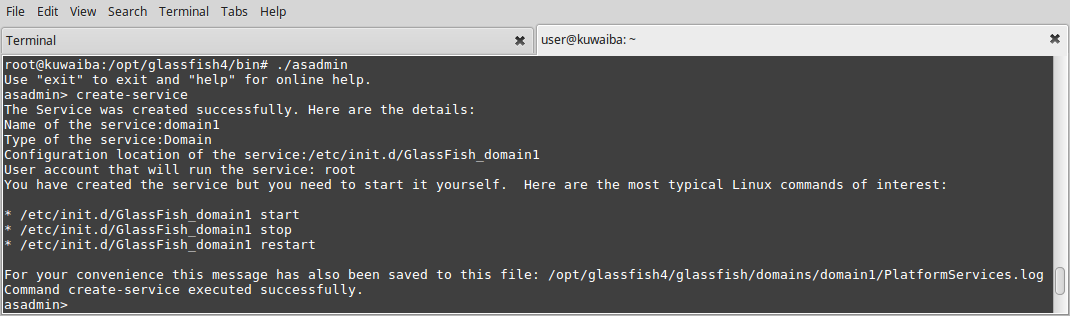
\includegraphics[width=1\linewidth]{img/glassfish_as_service_result.png}
			\caption{Setting up Glassfish as a service}
			\label{fig:glassfish_as_service_resultans}
		\end{figure}

	\section{Backup Script} \label{sec:backup_script}
		There is a script to make a backup of the kuwaiba's database and backgrounds, this script was put in the /etc/cron.daily/. It will made an incremental backup every Sunday, overwriting last Sundays backup, each incremental backup overwrites last weeks incremental backup of the same name. The script also made a full permanent backup on the 1st of every month.
	
	\section{Setup Glassfish} \label{sec:enable_https}
		\subsection{Server Port} To set the listener port for kuwaiba server in glassfish, you should go into the configuration file in your Glassfish domain folder \textit{/opt/glassfish4/glassfish/domains/domain1/config} and edit the line \textit{<network-listener port="8181" protocol="http-listener-2 transport="tcp" name="http-listener-2" thread-pool="http-thread-pool"></network-listener>}
		
		\subsection{Https in Client Side} If the https is enable in the server and you want logging using https in your client, you will need to get the file \textit{kuwaiba\_keystore.jks}, you will find this file in \textit{/data/installs/kuwaiba/dev/} (in the server were kuwaiba was deployed), once you have this file you must paste it in your local machine where you will run your client, to know where to paste this file you must go into your locally uncompressed client directory and look for \textit{kuwaiba/etc/\textbf{kuwaiba.conf}}, here you will find the right path to paste the \textit{kuwaiba\_keystore.jks}.
			
\end{document}